\section{Question 4}

\begin{question}
    Use your implementation of Newton's method to solve $f(x) = 0$ for 
\end{question}

I updated the function I used in question $3$ to output each p values and the functions evaluated at these p values.

\begin{verbatim}
    %% Updating the function newtonmethod
    % This function is almost the same as the newtonmethod except that this
    % method print out p and f(p) for each iteration
    function [p,iters] = newtonmethod2(f,df,p0)
        p = p0 - f(p0)./df(p0);
        iters = 0;
        while abs(p - p0) >= 10^(-10) && iters < 100
            p0 = p;
            p = p0 - f(p0)./df(p0);
            fp = f(p);
            iters = iters + 1;
            fprintf('p%d = %.10f\n', iters, p);
            fprintf('f(p%d) = %.10f\n', iters, fp);
        end
    end
\end{verbatim}

\subsection{Part a}

\begin{question}
    \item $f(x) = x^6+6x^5+9x^4-2x^3-6x^2$ with the initial starting points $-.75$ and $-2.2$. Output tables of each subsequent iteration (each $p$ value), and the function value of each $p$ value of the form \begin{tabular}{c|c} $p$ & $f(p)$ \\ \hline & \end{tabular} to evaluate convergence. What kind of convergence do you see here? 

\end{question}
    
\begin{answer}
    Using the \textit{newtonmethod2}, I test the function $f(x) = x^6+6x^5 + 9x^4 - 2x^3 -6x^2$ with initial guess of $-0.75$ and $-2.2$ separately. 
    \begin{verbatim}
        %% 4(a)
        fa = @(x) x^6 + 6*x^5 + 9*x^4 - 2*x^3 - 6*x^2;
        dfa = @(x) 6*x^5 + 30*x^4 + 36*x^3 -6*x^2 - 12*x;
        %[pa1, itera1] = newtonmethod2(fa,dfa,-0.75);
        %[pa2, itera2] = newtonmethod2(fa,dfa,-2.2);
    \end{verbatim}
    The initial guess of $-0.75$ gives me the result as shown in the Table \ref{tab:tab1}, and the initial guess of $-2.2$ gives me the result as shown in the Table \ref{tab:tab2}.
    \begin{table}[H]
    \parbox{.45\linewidth}{
    \centering
    \caption{Results for 4a with an initial guess of -0.75}
    \label{tab:tab1}
    \begin{tabular}{c|c}
    \textbf{p}                         & \textbf{f(p)}                    \\ \hline
    -1.0663512291                      & 0.4370293183                     \\ \hline
    -1.0053213226                      & 0.0321824778                     \\ \hline
    -1.0000417072                      & 0.0002502591                     \\ \hline
    -1.0000000026                      & 0.0000000157                     \\ \hline
    -1.0000000000                      & 0.0000000000                     \\ \hline
    \multicolumn{1}{l|}{-1.0000000000} & \multicolumn{1}{l}{0.0000000000}
    \end{tabular}
    }
    \hfill
    \parbox{.45\linewidth}{
    \centering
    \caption{Results for 4a with an initial guess of -2.2}
    \label{tab:tab2}
    \begin{tabular}{c|c}
    \textbf{p}                         & \textbf{f(p)}                    \\ \hline
    -3.0572164860                      & 1.3555436398                     \\ \hline
    -3.0116729699                      & 0.2229614374                     \\ \hline
    -3.0006442739                      & 0.0116355626                     \\ \hline
    -3.0000021337                      & 0.0000384066                     \\ \hline
    -3.0000000000                      & 0.0000000004                     \\ \hline
    \multicolumn{1}{l|}{-3.0000000000} & \multicolumn{1}{l}{0.0000000000}
    \end{tabular}
    }
    \end{table}
    Looking at the results given in the Table \ref{tab:tab1} and \ref{tab:tab2}, the function $f(x) = x^6+6x^5+9x^4-2x^3-6x^2$ converges quadratically.
\end{answer}

\subsection{Part b}

\begin{question}
    $f(x) = x^6+6x^5+9x^4-2x^3-6x^2+1$ with the initial starting points $-.75$ and $-2.2$. Output tables of each subsequent iteration (each $p$ value), and the function value of each $p$ value of the form \begin{tabular}{c|c} $p$ & $f(p)$ \\ \hline & \end{tabular} to evaluate convergence. What kind of convergence do you see here? 
\end{question}

\begin{answer}
    Similarly, if we implement the \textit{newtonmethod2} to the function $f(x) = x^6+6x^5+9x^4-2x^3-6x^2 + 1$ with initial guess of $-0.75$ and $-2.2$ separately.
    \begin{verbatim}
        %% 4(b)
        fb = @(x) x^6 + 6*x^5 + 9*x^4 - 2*x^3 - 6*x^2 + 1;
        dfb = @(x) 6*x^5 + 30*x^4 + 36*x^3 -6*x^2 - 12*x;
        %[pb1, iterb1] = newtonmethod2(fb,dfb,-0.75);
        [pb2, iterb2] = newtonmethod2(fb,dfb,-2.2);
    \end{verbatim}
    The initial guess of $-0.75$ gives me the result as shown in the Table \ref{tab:tab3}, and the initial guess of $-2.2$ gives me the result as shown in the Table \ref{tab:tab4}.
    \begin{table}[H]
    \parbox{.45\linewidth}{
    \centering
    \caption{Results for 4b with an initial guess of -0.75}
    \label{tab:tab3}
    \begin{tabular}{c|c}
    \textbf{p}                         & \textbf{f(p)}                    \\ \hline
    -0.6781724038                      & 0.0046036037                     \\ \hline
    -0.6655575336                      & 0.0011614860                     \\ \hline
    -0.6591620959                      & 0.0002917807                     \\ \hline
    -0.6559409638                      & 0.0000731271                     \\ \hline
    -0.6543243557                      & 0.0000183049                     \\ \hline
    \multicolumn{1}{l|}{-0.6535145166} & \multicolumn{1}{l}{0.0000045791} \\ \hline
    \multicolumn{1}{l|}{$\cdots$}      & \multicolumn{1}{l}{$\cdots$}    \\ \hline
    \multicolumn{1}{l|}{-0.6527036483} & \multicolumn{1}{l}{0.0000000000} \\ \hline
    \multicolumn{1}{l|}{-0.6527036483} & \multicolumn{1}{l}{0.0000000000}
    \end{tabular}
    }
    \hfill
    \parbox{.45\linewidth}{
    \centering
    \caption{Results for 4b with an initial guess of -2.2}
    \label{tab:tab4}
    \begin{tabular}{c|c}
    \textbf{p}                         & \textbf{f(p)}                    \\ \hline
    -3.1260289257                      & 4.9798681852                     \\ \hline
    -3.0203678242                      & 1.4061405106                     \\ \hline
    2.9562399979                       & 0.3813875294                     \\ \hline
    -2.9198296021                      & 0.1001816797                     \\ \hline
    -2.9001879500                      & 0.0257512145                     \\ \hline
    \multicolumn{1}{l|}{-2.8899435089} & \multicolumn{1}{l}{0.0065339926} \\ \hline
    \multicolumn{1}{l|}{$\cdots$}      & \multicolumn{1}{l}{$\cdots$}               
    \end{tabular}
    }
    \end{table}
    The number of iteration is $100$ when we use the initial guess of $-2.2$ as shown in the Figure. \ref{fig:fig2}
    \begin{figure}[H]
        \centering
        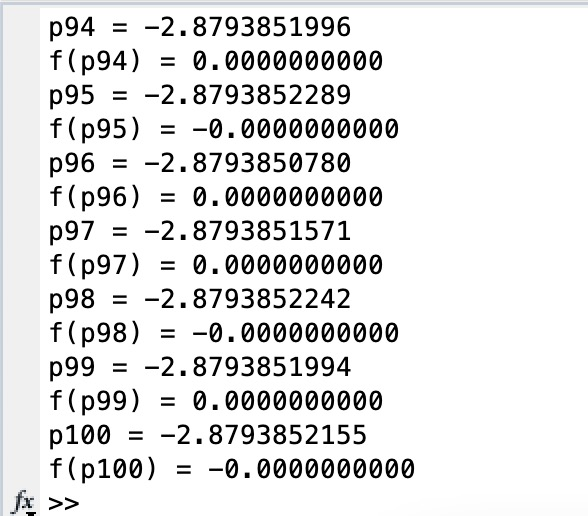
\includegraphics[width=0.5\textwidth]{Figure 2.png}
        \caption{\label{fig:fig2}Result of implementing the newtonmethod2 with initial guess of -2.2}
    \end{figure}
    Thus, the function $f(x) = x^6+6x^5+9x^4-2x^3-6x^2 + 1$ actually diverges.
\end{answer}

\subsection{Part c}

\begin{question}
    Why is the convergence different between the two functions?
\end{question}

\begin{answer}
    The reason why the $f(x) = x^6+6x^5+9x^4-2x^3-6x^2$ converges, while $f(x) = x^6+6x^5+9x^4-2x^3-6x^2 + 1$ converges with initial guess of $-2.2$ is that the initial guess is too far away from the real zero of the function $f(x) = x^6+6x^5+9x^4-2x^3-6x^2 + 1$.
\end{answer}